\chapter{Background and Terminology}
Network telescope is responsible for capturing data from nefarious and potentially malicious traffic found on the internet.
The obtained dataset is analysed by making use of set of specific rules and utilize them to gather necessary information.
This information has to be made use of in an efficient manner.
By plotting the diagrams, one can decipher and comprehend what the information represents.
This thesis involves the gathering of such information, analysing and visualizing it by plotting the graphs.\\\\
One of the reasons for the anomalous unsolicited traffic are malicious network scans.
Scans are used to locate vulnerable computers in the network by automated or manual attempts from the user.
Internet threat monitors continuously observe many types of scans including methodical scans targeting single or multiple ports successively through an IP address range, continuous scans of ports on a single IP address and even ping based scans to check whether the device is existing on a given IP address.\\\\
This chapter will discuss the concept of network telescope, internet scanner (port scanner), honeypots and other related concepts which will be essential for the better understanding of rest of the paper.
    \section{TCP 3-way Handshake Process}
    Before discussing about Internet scanner and different types of port scanning methods, it is desire to have a basic knowledge about how TCP setup a TCP/IP connection over an Internet Protocol based network.
    TCP is one of the important protocols of the TCP/IP suite.
    It is connection oriented protocol as it provides reliable, error free, ordered communication between two hosts in a network.
    In order to provide the features mentioned above to the applications, it setup communication between the two devices that wish to communicate.
    This procedure typically called connection establishment, includes a trade of messages that moves both devices from their initial connection state (CLOSED) to the normal operating state (ESTABLISHED) \cite{rfc761}.
    \begin{figure}[t]
    \centering
	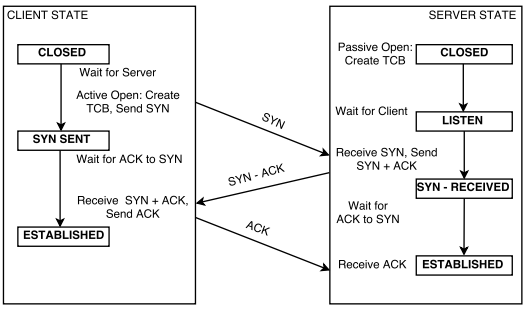
\includegraphics[width=10cm, height=6cm]{images/tcp_handshake.png}
	\caption{TCP 3-Way Connection Establishment Procedure}
	\end{figure}
	\\\\
	Figure 2.1 illustrates how the connection is established between two applications.
	TCP maintains data about each connection separately.
	This can be achieved by TCP with a special data structure called transmission control block (TCB).
	Before the process of setting up a TCP connection can begin, client and server create TCB to hold the information about it.
	To establish a connection between two devices, they should both send a SYN message and receive ACK for it.
	So the connection establishment involves three steps.
	Initially client sends a SYN message to the server. 
	Server sends the message that combines the ACK message for the client's SYN and SYN message for client.
	Finally client acknowledges the SYN message of server by sending an ACK to server.
	Thus connection is established between two devices.
	\section{Internet Scanner}
	Network scanning is a powerful tool utilized by analysts to study and measure the Internet and by attackers to enumerate vulnerable targets.
	There are two kinds of port scanning approaches existing nowadays: horizontal scanning which targets single port (process of scanning large number of hosts on a single port) and scans distributed across infected botnet hosts \cite{allman2007brief}\cite{dainotti2012analysis}\cite{czyz2013understanding}\cite{pang2004characteristics}.
	The idea of Internet scanners evolved during the late 90's by the initial release of NMap scanner \cite{lyon2009nmap}.
	After that many researches have been taken place in this field and many Internet scanners have been implemented.
	While well popular scanners like NMap provides many features like port scanning, host discovery, OS detection, it requires months to complete full scan over the Internet.
	However high speed Internet scanners like ZMap \cite{durumeric2013zmap} and Masscan \cite{graham2014masscan} take only few minutes to scan the entire IPv4 address space\\\\	
	As mentioned before, several Internet scanners are available such as ZMap, Masscan and NMap.
	Each of these scanners shows different characteristics based on their motives and how it is implemented.
	Since ZMap is currently one of the most well known Internet scanners, we choose it to explain the general working methodology of such scanners.
	ZMap \cite{durumeric2013zmap} is a high speed Internet-wide scanning tool which was developed by set of computer scientists from University of Michigan.
	One of the main advantages of ZMap is, it is able to complete a scan which targets at particular port or service of whole Internet from a dedicated computer in less than 60 minutes.
	It has one programming segment which sends the packets by using raw network sockets, thus cleverly avoids any overheads of the TCP stack.
	And another segment is used to gather and save any responses.
	Moreover ZMap allows to send more than 1 million probe packets at every second by bypassing the TCP stack, and a \SI{1}Gbit/sec outbound connections.
	\subsection{How ZMap differs from other scanners}
	In other network scanners like NMap, the Ethernet frame send by the users will be delivered to the target system much slower than high speed scanners, as well as the replies to source address.
	This is  due to the presence of network protocol overhead and inefficient method to avoid saturating the source or target networks.
	NMap scans the entire IP address range in numerical address sequence as well as it sends the packet to each IP address and waits for a reply.
	It also maintains state for each connection to keep track of previous scans and to deal with re-transmission and timeouts.
	As a result, there is a high probability of network congestion in the network being examined, thus resulting in a Denial of Service (DoS).\\\\
	ZMap tackled this issue by utilizing a technique called cyclic multiplicative groups.
	ZMap uses an iterative formula to visit every whole number from 1 to {$2^{32}$ – 1} (zero is omitted) at once, in a pseudo random order.
	So the probability of targeting single subnet at the same time during huge number of tests is lower.
	In view of this reason, ZMap does not make any part of the network busy or cluster the traffic in any part of the web.
	ZMap does not re-transmit the packets to avoid keeping the state, as it always sends a constant number of probes per target.
	Moreover ZMap is equipped for scanning the whole IPv4 addresses 1300 times quicker than Nmap's most proficient scanning setting.
	\subsection{How Internet scanners hide port scanning activity}
	Due to security concerns, organizations started deploying network security mechanisms such as firewalls to reduce the network activity.
	After the wide use of Internet scanners, people began adding the security features to firewalls to detect and block port scanning activity.\\\\
	Nevertheless, Internet scanners use variety of methods to obscure the port scanning activity, thus evade the detection of port scanning mechanisms. 
    For instance, Nmap provides its customers the ability to change the order of and timing between packets and randomize destination IPs \cite{lee2003detection}.
    It allows users to randomize each group of up to 16384 hosts before it scans them.
    This can make the scanning activity less evident to different network security systems, particularly when it combines with slow timing options \cite{nmap1}.\\\\
    Another way to avoid the detection is to use spoofed IP or IP decoys to conceal the attacker's IP address.
    Internet scanners enable users to use spoofed IPs to spoof the scan to make the targets believe that another person is scanning them.
    Furthermore, it permits to use IP decoys to perform decoy scan, which give a feeling to the remote target that the IP addresses you specify as decoys are scanning the target network as well \cite{nmap1}. 
    It results to make network monitoring systems behave like, it reports multiple scans from the same IP address. 
    Hence they cannot understand which IP was scanning them and which were innocent decoys.
    \subsection{Scanning Methods}
    Port scanning tools are widely used by attackers to identify the vulnerable ports and network administrators to study and correct the weakness in their own administrated network.
    Port scans often consider as the elementary step for attackers to find the vulnerable hosts or network and get access to it.
    Attackers use different scanning methods to scan the target hosts or network, to understand which service can be exploited to get the necessary information. 
    Port scan tools offer different scan techniques and users can choose the appropriate one according to their purpose.\\\\
    Selecting the appropriate scan methods is one of the most important decisions a user has to make while planning port scan attacks.
    Port scanning tool provides several port scanning techniques that gives the client the flexibility to create scans which might be more appropriate than using other techniques.
    Different types of port scanning techniques are listed below.\\\\
    \textbf{TCP SYN scan} -  SYN scan is relative simple and quick scan and can scan a large number of ports in every  seconds. 
    Figure 2.2 shows the process of TCP SYN scan  of an open port on the left, and of a closed port on the right.
    \begin{figure}[t]
    \centering
	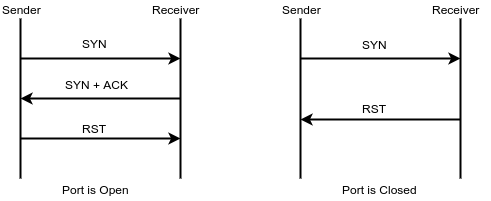
\includegraphics[width=10cm, height=6cm]{images/tcp_synscan.png}
	\caption{TCP SYN Scan Process}
	\end{figure}
    It  works  in  such  a  way  that  it  does not  finish  the  3-way  TCP  handshake mechanism.  
    It  just  sends  an  initial  SYN  signal  and  wait  for  the  SYN-ACK  message from  the  target.
    If the sender receives the SYN-ACK message, it sends RST message to the target and connection is not established.
    However, if the port is closed, target system sends RST message to the sender.
    Since it does not establish the connection, it is also known as TCP half open scan.\\\\
    \textbf{TCP Connect scan} -  TCP  connect  scan  is resource sensitive and slower scan compared to TCP half open scan.  It completes the handshake mechanism and establish a connection by sending the ACK packet, but close the connection just after it.
    As the target system assign resources to enable the TCP connections during TCP connect scan, it can cause performance issues on the target system.
    In addition to that, this sort of scan is easily detectable and filterable.\\\\
    \textbf{TCP NULL, XMAS, FIN scan} - Another approach to utilize the TCP protocol to gain information about the target system are TCP Null, Xmas, FIN scan. 
    These scanning methods are known as stealth scans, as TCP header flags are setup in such a way that it will gain necessary information back from target system without attempting for connection establishment or establishing the connection.
    It differs from the TCP SYN and connect scan as it attempts to collect the information during  TCP three way handshake process.
    While TCP Null, FIN and Xmas scans analyze the packets, which
    follow to the corresponding packets sent from the scanner to the scans victim.\\\\
    The null scan does not set any bits and its TCP header flag will be empty.
    If the port is open, these packets will be ignored by the target system as these packets are invalid and would never occur in the real world.
    However, if the port is closed, sender receives a RST packet as the port is unreachable.\\\\
    The FIN scan sends the packet by just setting the FIN flag in the TCP header to the target system.
    This kind of TCP packets are generally used to terminate an established connection.
    If the port in the target system is closed and it receives the FIN packet without establishing a connection with sender, it reacts with a RST packet.
    If sender does not receive any response from host system, the port is considered open.\\\\
    During Xmas scan the port scanner sends TCP packets in which FIN, PSH (PUSH) and URG (Urgent) flags in the TCP header are set \cite{port_techniques}.
    The URG flag is used to inform a receiving station that certain data within a segment is urgent and should be prioritized.
    The PSH flag in the TCP header informs the receiving host that the data should be pushed up to the receiving application immediately.
    If the sender does not receive any response to the packet from the target system, the port is considered open and if a RST packet is received, the port is considered closed.\\\\
    \textbf{UDP scans} - UDP port scans are another type of port scanning activity which is based on UDP protocol.
    Since UDP is a connection-less protocol, UDP scanning is generally slower and difficult to implement than TCP.
    UDP scan works by sending an UDP packet to every targeted port.
    If the destination port is closed, the system will respond with ICMP port unreachable error (type 3, code 3) message.
    If no response is received after sending the packet, the port is considered as open.
    It generally re-transmit the packets to ensure that packet is not lost while transmission thereby reaffirm port is open.
    However, if port is filtered by a firewall, this method will falsely report that port is open \cite{de1999review}.\\\\
    Another approach is to send packet with protocol-specific payload to some common destination ports to increase response rate.
    This method is much more reliable at identifying open ports.
    However, it is limited to scanning some common ports for which an application probe packet is available.
    Some port scanners such as nmap generally have probes for less than 20 UDP services, while some commercial tools (e.g., nessus) have as many as 70. In some cases, a service may be listening on the port, but configured not to respond to the particular probe packet \cite{port_techniques}. 
	\section{Network Telescope}
	The idea of Network Telescopes as a method for monitoring activity on the Internet everywhere, has grown progressively since mid 2000.
	Network Telescope is a tool that monitors traffic destined to what is known as "Internet dark address space".
	These addresses are portion of routed, allocated IP address space in which no active services or servers reside.
	Since no legitimate packets travel through these address spaces, one can obtain information about possible network attacks as well as misconfigurations by watching the network traffic addressed to these IP addresses.
	Network Telescope  mostly carries  illegitimate traffic such as continuous view of anomalous unsolicited traffic, or Internet Background Radiation (IBR).
	IBR emerges from an extensive variety of events, such as backscatter resulted from spoofing, misconfigurations, scanning of IP address space by attackers or malware looking for vulnerable targets, and Internet worms.\\\\
	Traffic originating from Internet hosts and are received by network telescope can be classified as one of the following three broad categories:
	\begin{itemize}
	\item Backscatter - The traffic resulting because of the victims response to the spoofed packets as normally it would respond to the legitimate requests.
	This traffic comprises fundamentally of specific classes of ICMP traffic and of TCP packets with RST (reset) or SYN (synchronise) and ACK (acknowledgement) flags set.
	\item Configuration Mistakes - A traffic flow which occur due to the misconfiguration of the computers in the Internet. 
	This flow lives only for a short period of time.
	\item Host/Port scanning - The traffic that can be grouped as being originated from different scanning agents like ZMAP, NMAP, Massscan etc.
	\end{itemize} 
    Network telescope can be categorized in to mainly two: active and passive network telescope.
    Passive network telescope is able to capture the incoming packets, however is unable to respond to these packets.
    Active network telescope responds to the incoming packets and try to establish the connection using 3-way TCP handshake.
    \subsubsection{Passive Network Telescope}
    Passive network telescope observes the network traffic targeting the address space of the network but is insufficient to respond to any of the incoming packets.
    It is unable to complete the 3-way TCP handshake which is the requirement for starting the actual transmission of TCP data.
    However it is able to receive the payload data from UDP and ICMP packets as they are connection less protocols.
    \subsubsection{Active Network Telescope}
    Active network telescope is able to respond to the incoming connection requests captured by it.
    It can respond to the 3-way TCP handshake mechanism thus able to receive the TCP payload from the remote connections.
    A responder replies to a TCP SYN request with a TCP SYN-ACK packet and in so doing receive the first packet containing a data payload \cite{bailey2006practical}.
    Thus actual data can be used to get a better understanding about the remote connections.
	\subsection{The Case for Monitoring}
	Nowadays, it is essential to find a solution to understand  and respond to rising dangers in the Internet.
	Data security specialists both in the scholarly community and at security sellers first need to be capable to isolate and study both the behaviours of the actual binary files associated, but also the behavioral perspectives related to the worldwide system-the Internet.
	The monitoring of network services can be categorised in to two main types:
	\begin{itemize}
	    \item Passive Monitoring - One of the greatest issues with conventional monitoring schemes is the issue of differentiating between legitimate and unexpected traffic.
	    The utilization of network telescopes to tackle the monitoring issues above, can in some ways alleviate these difficulties.
	    This can be accomplished, by observing just the activity that is not part of legitimate traffic,  and therefore already potentially suspect. 

	    \item Distributed Monitoring - The importance of monitoring the networks has been increased inspired the implementation of the distributed networking.
	    It consists of  multiple smaller sensors or alternately a single sensor with multiple smaller address allocations to monitor.
	    Distributed monitoring makes sense, if an organisation has larger address space, or sufficiently fortunate to have numerically non-contiguous address space.
	\end{itemize}
    There may be some security concerns within an organisation when a network telescope is established.
    Some of the potential threats to passive sensors are discussed in the \cite{shinoda2005vulnerabilities}.
    Considering this, an accurately configured framework ought to prove an advantage for an association's Information Security toolset, instead of a risk.
    \subsection{Analysis of Network Telescope Traffic}
    Packets received by the network telescope can be classified as internet worms, backscatter resulted from spoofing, misconfigurations, scanning of IP address space by attackers or malware looking for vulnerable targets.
    These packets should be analysed carefully to understand the motive behind each packet.
    However this can be identified easily by just understanding the traffic and how it is generated.
    \begin{table}[t!]
    \centering
    \begin{tabular}{ |p{6cm}|p{6cm}|  }
    \hline
    Packet sent & Response from destination\\
    \hline
    TCP SYN (open port)   & TCP SYN/ACK\\
    TCP SYN (closed port) & TCP RST\\
    TCP RST & no response\\
    TCP ACK    &  TCP RST\\
    TCP NULL & TCP RST (ACK)\\
    UDP packet (open port)& Protocol Dependent\\
    UDP packet (closed port)& ICMP Port Uncreachable\\
    ICMP Echo Request & ICMP Echo Reply\\
    ICMP TS Request & ICMP TS Reply\\
    \hline
    \end{tabular}
    \caption{Packet Requests and Responses \cite{moore2006inferring}}
    \end{table}
    \\\\
    Each type of attack uses different mechanism to achieve its goal. 
    For example, the motive behind the DoS attacks is to consume the resource of its target, that can be a host or a network.
    To achieve that, SYN Flood mechanism is used where several SYN packets are sent continuously.
    For each SYN packet received by the destination host, it has to process that packet by storing the information about the connection requests, thus consume the resources of the host.
    These mechanisms are mostly influenced by the way the packet is requested and its response.
    The Table 2.1 shows the common packet requests and their responses.
    \subsection{Internet Threat Monitor}
	Due to the significance and usefulness of network telescopes, numerous projects and collective efforts have been taken place to explore the field of network monitoring.
	CAIDA, the Cooperative Association for Internet Data Analysis \cite{caida} started one of the initial works in the field of network monitoring and they use network telescope which is huge, routed, but very sparsely populated address block. 
    DShield \cite{dshield} a community-based collaborative firewall log correlation system took an another approach that collects firewall logs from participating system administrators.
    Many such monitoring systems have been deployed around the world due to the success of these systems.
    These systems can be commonly referred to as Internet threat monitors.
    \begin{figure}[t]
    \centering
	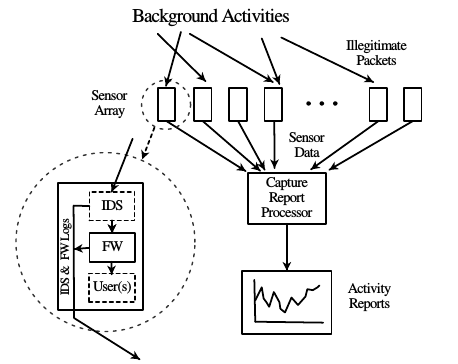
\includegraphics[width=8cm, height=6cm]{images/int_threat_mon}
	\caption{ Structure of a Typical Internet Threat Monitor \protect\cite{caida}}
	\end{figure}
	\\\\
	A typical Internet threat monitor can be seen in the Figure 2.3. 
	It comprises set of sensors listening to packets arriving at a set of IP addresses, capturing all traffic sent to these addresses.
	Sensors can be categorized in to passive and active based on the traffic it receives and how it responds to it.
	A passive sensor is configured to receive IBR traffic and no legitimate response is sent back to source.
	As such, it is difficult for a potential attacker or instance of malware to determine anything about the target system.
	Moreover since it does not reply to any incoming packets, it requires significantly less computing and bandwidth resources than active sensor.
	An active sensor replies to incoming IBR traffic to solicit further  traffic  so  as  to  more  precisely detect  its  nature  and intent.
	Examples include Internet motion sensor \cite{cooke2004internet} and honeypots.
	Server is the place where all data collected by the sensors is  stored, processed, analyzed and presented.
    \section{Honeypots}
    Honeypot is a computer security mechanism set to act as a decoy to attract malicious traffic.
    The main purpose of the honeypot is to detect, deflect and investigate the attempts to gain illegitimate access to information systems \cite{provos2004virtual}.
    It comprises a computer, applications, and information that reproduce the behavior of a genuine system that gives off an impression of being a piece of a system but is really detached and closely observed.\\\\
    Honeypots are similar in character to network telescopes.
    Both can be used to monitor the individual or range of IP addresses to capture the nefarious traffic.
    However the honeypot differs from network telescope regarding the method of capturing the  malicious packets.
    Honeypots actively communicate with a threat and attract the malicious traffic whereas network telescope just listens to the incoming traffic. 
    This enables honeypots to describe  the vulnerability that has been exploited and its effect on a machine \cite{bailey2005data}.\\\\
    Honeypots can be categorized in to mainly two based on its design criteria: low and high interaction honeypot.
    The low interaction honeypot emulates just services often requested by the 
    attackers, while a high interaction honeypot reproduces the behavior of a complete physical machine that host different services.
    By using honeypot, it is possible to learn more about the behavior of  different attacks such as how an attacker exploits the vulnerabilities in the system to  gain root access of the host.
    \section{Network Packet Analysing Tools}
    During the course of thesis, different packet analysing tools were used in order to analyse the capture files.
    It can be used to analyse the network traffic and generated customized report to assist researchers or organization in managing their networks.
    This section briefly explains the tools that were used during the thesis work.
    \subsection{Wireshark}
    Wireshark was developed in 1998 and is one of the widely used packet analyser in the world \cite{wireshark}.
    Wireshark provides a significantly more full highlighted graphical environment in which one can perform more useful analysis and filtering of the packets.
    It can be also used to dissect the part of the protocol and subsequently decoding the information for an encapsulated higher order protocols.
    Wireshark support libpcap file format (also known as pcap file format) which is popular file format for storing, reading and interchange of packet data.
    The biggest problem experienced with Wireshark is the inefficiency to load and work with files containing large number of packets.
    \subsection{Tshark}
    TShark is another version of Wireshark which is purely terminal based, works similar to tcpdump, but more powerful than it \cite{tshark}.
    It is used for capturing and filtering out packets when an interactive user interface is not accessible or required. 
    The two primary benefits of Tshark are that it can be used  on a remote computer through a SSH connection and as a part of scripts.
    